% Escolha: Portugues ou Ingles ou Espanhol.
% Para a versão final do texto, após a defesa, acrescente Final:

\documentclass[Portugues]{phdquali}
%\documentclass[Portugues,Final]{phdquali}

\usepackage[latin1,utf8]{inputenc}

% Para identar primeiro parágrafo:
\usepackage{indentfirst}

% Para acrescentar comentários ao PDF descomente:
\usepackage
%  [pdfauthor={nome do autor},
%   pdftitle={titulo},
%   pdfkeywords={palavra-chave, palavra-chave},
%   pdfproducer={Latex with hyperref},
%   pdfcreator={pdflatex}]
{hyperref}

\def\ie{i.e.\onedot} \def\Ie{I.e.\onedot}
\def\eg{e.g.\onedot} \def\Eg{E.g.\onedot}

\begin{document}

% Escolha entre autor ou autora:
\autor{João Victor da Silva Guerra}
%\autora{Nome da Autora}

% Sempre deve haver um título em português:
\titulo{Desenvolvimento de plataforma de metodologias computacionais para caracterização estrutural e funcional de biomoléculas e sítios de ligação}

% Se a língua for o inglês ou o espanhol defina:
%\title{The Dissertation or Thesis Title in English or Spanish}

% Escolha entre orientador ou orientadora. Inclua os títulos acadêmicos:
\orientador{Prof. Dr. Paulo Sergio Lopes-de-Oliveira}
%\orientadora{Profa. Dra. Nome da Orientadora}

% Escolha entre coorientador ou coorientadora, se houver.  Inclua os títulos acadêmicos:
%\coorientador{Prof. Dr. Eng. Lic. Nome do Co-Orientador}
%\coorientadora{Profa. Dra. Eng. Lic. Nome da Co-Orientadora}

% Escolha entre mestrado ou doutorado:
% \mestrado
\doutorado

% Se houve cotutela, defina:
%\cotutela{Universidade Nova de Plutão}

\datadadefesa{01}{01}{2023}

% Para a versão final defina:
%\avaliadorA{Prof. Dr. Primeiro Avaliador}{Instituição do primeiro avaliador}
%\avaliadorB{Profa. Dra. Segunda Avaliadora}{Instituição da segunda avaliadora}
%\avaliadorC{Dr. Terceiro Avaliador}{Instituição do terceiro avaliador}
%\avaliadorD{Prof. Dr. Quarto Avaliador}{Instituição do quarto avaliador}
%\avaliadorE{Prof. Dr. Quinto Avaliador}{Instituição do quinto avaliador}
%\avaliadorF{Prof. Dr. Sexto Avaliador}{Instituição do sexto avaliador}
%\avaliadorG{Prof. Dr. Sétimo Avaliador}{Instituição do sétimo avaliador}
%\avaliadorH{Prof. Dr. Oitavo Avaliador}{Instituição do oitavo avaliador}


% Para incluir a ficha catalográfica em PDF na versão final, descomente e ajuste:
%\fichacatalografica{arquivo.pdf}


% Este comando deve ficar aqui:
\paginasiniciais


% Se houver dedicatória, descomente:
%\prefacesection{Dedicatória}
%A dedicatória deve ocupar uma única página.


% Se houver epígrafe, descomente e edite:
% \begin{epigrafe}
% {\it
% Vita brevis,\\
% ars longa,\\
% occasio praeceps,\\
% experimentum periculosum,\\
% iudicium difficile.}
%
% \hfill (Hippocrates)
% \end{epigrafe}


% Agradecimentos ou Acknowledgements ou Agradecimientos
\prefacesection{Agradecimentos}

Gostaria de expressar meus sinceros agradecimentos a todos que me apoiaram durante o desenvolvimento deste projeto. Em primeiro lugar, sou grato aos meus pais, Roseli do Carmo Freitas da Silva e Mario Luiz da Silva Guerra, por me apoiarem em todas as etapas da minha formação acadêmica e profissional. Agradeço à minha companheira, Bruna Martins da Silva, pelo apoio incondicional em todas as fases deste projeto.

Gostaria de agradecer ao meu orientador, Dr. Paulo Sergio Lopes de Oliveira, por ter me dado liberdade científica e criativa para desenvolver esta tese e, acima de tudo, pela oportunidade de trabalhar em um centro de pesquisa de excelência. Agradeço aos meus colegas do Laboratório de Biologia Computacional, José Geraldo de Carvalho Pereira, Helder Veras Ribeiro Filho, Luiz Fernando Giolo Alves, Mariana Bortoletto Grizante, Gabriel Ernesto Jara e Leandro Oliveira Bortot, por terem me apoiado em momentos importantes, compartilhando ideias e sugestões para o desenvolvimento deste projeto. Sou imensamente grato a todos que me ajudaram nesta etapa essencial da minha formação acadêmica.

Por fim, gostaria de agradecer ao Programa de Pós-Graduação em Ciências Farmacêuticas da Faculdade de Ciências Farmacêuticas da Universidade Estadual de Campinas, ao Laboratório Nacional de Biociências e ao Centro Nacional de Pesquisa em Energia e Materiais, por terem viabilizado este trabalho. Também sou grato pelo apoio financeiro da Fundação de Amparo à Pesquisa do Estado de São Paulo (FAPESP) pelo projeto de pesquisa regular (processo nº 2018/00629-0, Fundação de Amparo à Pesquisa do Estado de São Paulo (FAPESP))."


% Sempre deve haver um resumo em português:
\begin{resumo}
O resumo deve ter no máximo 500 palavras e deve ocupar uma única página.
\end{resumo}


% Sempre deve haver um abstract:
\begin{abstract}
The abstract must have at most 500 words and must fit in a single page.
\end{abstract}


% Se houver um resumo em espanhol, descomente:
%\begin{resumen}
% A mesma regra aplica-se.
%\end{resumen}


% A lista de figuras é opcional:
\listoffigures

% A lista de tabelas é opcional:
\listoftables

% A lista de abreviações e siglas é opcional:
% \prefacesection{Lista de Abreviações e Siglas}

% A lista de símbolos é opcional:
% \prefacesection{Lista de Símbolos}

% Quem usa o pacote nomencl pode incluir:
% \renewcommand{\nomname}{Lista de Abreviações e Siglas}
%\printnomenclature[3cm]


% O sumário vem aqui:
\tableofcontents


% E esta linha deve ficar bem aqui:
\fimdaspaginasiniciais

% O corpo da dissertação ou tese começa aqui:

%%% Chapter 1

\chapter{Introdução}

% \begin{itemize}
%  \item Comece explicando a importância dos sítios de ligação em biomoléculas e como eles afetam a função biológica das moléculas;
%  \item Apresente os métodos experimentais e computacionais disponíveis para identificar e caracterizar sítios de ligação;
%  \item Descreva brevemente os programas computacionais mais utilizados na área e suas principais características;
%  \item Finalize apresentando o objetivo e a estrutura do seu trabalho.
% \end{itemize}

Biomoléculas, como proteínas e ácidos núcleios, são moléculas complexas que desempenham funções biológicas essenciais para a vida. Processos biológicos, como a transdução de sinal, a integridade estrutural, a adesão celular e a apoptose, são modulados por interações biomoleculares \cite{sotriffer2002,henrich2010}. Essas interações são extremamente importantes para a compreensão de processo biológicos e para o desenvolvimento e/ou aprimoramento de terapias farmacológicas \cite{henrich2010}. No entanto, os estudos dos mecanismos intrínsicos dessas interações ou possíveis pontos de interação são desafiadores, devido à complexidade das biomoléculas e à diversidade das interações que ocorrem entre elas.

Usualmente, essas interações ocorrem entre os receptores e ligantes, que variam de íons, como ferro e fosfato, a macromoléculas, como proteínas, RNA e DNA \cite{oliveira2014}. Para execução dessas interações, estruturas atomísticas se dobram orquestradamente para criar sítios de ligação específicos, comumente localizados em cavidades ao longo da superfície molecular, expondo padrões topológicos e físico-químicos para acomodar ligantes específicos \cite{henrich2010,guerra2021}. As interações receptor-ligante, como interações proteína-proteína (IPP), proteína-ligante (IPL), proteína-RNA (IPR) e proteína-DNA (IPD), são consequência da complementariedade entre as superfícies moleculares do par de interação, restringindo assim a um pequeno número de ligantes a interação eficiente com um dado receptor \cite{henrich2010,simoes2017}.

Dada a importância das interações biomoleculares, o estudo das biomoléculas e seus sítios de ligação são essencias para compreensão de processos biológicos e para o aprimoramento e desenvolvimento de novos fármacos. A utilização de abordagens computacionais para identificar sítios de ligação e caracterizar interações biomoleculares tem se mostrado uma alternativa eficaz para complementar os métodos experimentais e fornecer informações detalhadas sobre as interações moleculares \cite{simoes2017}. A identificação de sítios de ligação é um problema de classificação, onde o objetivo é determinar se um dado ponto na superfície de uma biomolécula é um sítio de ligação ou não \cite{sotriffer2002,henrich2010,simoes2017}. Enquanto isso, avanços em recursos computacionais e base de dados têm impulsionado o uso de métodos \textit{in silico} para simular a dinâmica de biomoléculas e implementar aplicações de inteligência artificial para estudar estruturas biomoleculares \cite{tunyasuvunakool2021}. Juntos, todos esses dados estruturais fornecem terreno fértil para interpretação de dados por meio de ciência de dados ou protocolos automatizadas, mas a análise intensiva de dados requer rotinas eficientes e integráveis com uma estrutura de dados facilmente manipulável.

Nesse cenário, ainda há a necessidade de ferramentas computacionais robustas e abrangentes para estudos computacionais de sistemas biomoleculares, capazes de cobrir as diferentes formas de interação. Ferramentas que sirvam como blocos de construção, para aplicações, programas e/ou protocolos automatizados de biologia computacional, biologia estrutural, aprendizado de máquina e áreas correlatas, são essenciais para análise de biomoléculas e/ou sítios de ligação. O desenvolvimento de ferramentas que possam ser utilizadas em diferentes tipos de aplicações e potencialidades é de suma importância nesse contexto.

Nesse sentido, o KVFinder suite é uma plataforma computacional que tem como objetivo atender a essas demandas. O KVFinder suite é composto por um conjunto de ferramentas para codificação e caracterização de biomoléculas e detecção e caracterização de sítios de ligação nessas biomoléculas. O KVFinder suite é composto por cinco ferramentas: parKVFinder \cite{guerra2020}, pyKVFinder \cite{guerra2021}, KVFinder-web \cite{guerra2023A}, KVFinderMD e SERD. Essa plataforma tem o potencial de ser uma ferramenta robusta e abrangente para estudos computacionais de sistemas biomoleculares, e pode ser utilizada em diferentes aplicações e contextos, desde a biologia estrutural até a ciência de dados.


\section{Identificação de sítios de ligação em biomoléculas}

Ao longo das últimas décadas, diversas abordagens \textit{in silico} foram desenvolvidas para identificação de sítios de ligação em proteínas para aprofundar os conhecimentos acerca de função de uma determinada proteína e para descoberta e melhoramento de fármacos \cite{liang1998}. No entanto, apenas algumas metodologias são aplicáveis à outros tipos de biomoléculas, \eg, ácidos núcleicos, carboidratos e lípideos. As abordagens computacionais publicados podem ser divididos em três categorias principais: geométricas, energéticas e evolutivas \cite{oliveira2014,simoes2017}.

\begin{itemize}
  \item \textbf{Métodos evolutivos:} são baseados na busca por resíduos conservados em alinhamentos de sequências múltiplas e informações de perfis conhecidos de sítios de ligação;
  \item \textbf{Métodos energéticos:} identificam sítios de ligação a partir da interação energética entre a biomolécula-alvo e uma sonda química, geralmente um grupo químico;
  \item \textbf{Métodos geométricos:} identificam cavidades analisando as características geométricas da superfície molecular.
\end{itemize}

Cada categoria de métodos possui seus próprios benefícios e desvantagens. Algoritmos evolutivos dependem fortemente de informações de sequência ou bancos de dados de sítios de ligação ativos e da qualidade do procedimento de alinhamento, enquanto os métodos energéticos dependem de procedimentos de filtragem, parametrizações de campo de força e funções de pontuação utilizadas. Por outro lado, métodos de detecção geométrica são relativamente simples e diretos e não exigem nenhum conhecimento não geométrico, apenas dados estruturais da proteína, \ie o arquivo no formato PDB, XYZ, mmCIF ou equivalente, contendo as coordenadas cartesianas dos átomos, que podem ser facilmente acessadas no Worldwide Protein Data Bank (wwPDB). Uma vez que as coordenadas dos átomos estão disponíveis, métodos geométricos devem ser capazes de representar qualquer tipo de biomolécula. Embora métodos puramente geométricos sejam eficientes na identificação de todos os tipos de cavidades de uma molécula alvo, identificar aquelas que são funcionalmente relevantes apresenta um problema. No entanto, a caracterização de cavidades em termos de propriedades físico-químicas bem escolhidas pode levar à identificação de cavidades funcionalmente relevantes, ou seja, sítios de ligação para um conjunto específico de ligantes.

Em geral, algoritmos baseados em geometria são os mais frequentemente usados para detectar cavidades em proteínas. Enquanto métodos baseados em evolução seriam limitados a proteínas porque dependem de princípios da evolução biológica, métodos baseados em energia poderiam ser aplicáveis, mas exigiriam ajustes finos dos parâmetros de campo de força adaptados à outros tipos de biomoléculas. Como ácidos núcleicos, carboidratos e lipídeos podem ter propriedades distintas em comparação com proteínas, métodos que dependem apenas de informações geométricas (por exemplo, coordenadas Cartesianas em 3D e tamanho do átomo) são desejáveis.

% pro e contra

\subsection{Abordagens geométricas}

% Geometric approaches for cavity detection have been vastly employed, which has a wide range of different techniques [3,18]. Since these techniques are relatively simple, straightforward and do not rely on prior knowledge, the approach is the most recurrent in the literature [1,5]. Here, we briefly present a comprehensive classification on geometry-based cavity detection approaches, whose taxonomy include grid-, sphere-, tessellation- and surface-based techniques, and combinations of those [3,18].

\subsection{Ferramentas disponíveis para detecção e caracterização de sítios de ligação}

\begin{itemize}
  \item KVFinder, parKVFinder, pyKVFinder
  \item Fpocket
  \item CAVER
  \item GHECOM
\end{itemize}

% Cavity characterization 

%%% Chapter 2

\chapter{Objetivos}

\section{Objetivo geral}

Este trabalho tem como objetivo o desenvolvimento de uma plataforma computacional, denominada \textbf{KVFinder suite}, para estudo de sistemas biomoleculares em biologia estrutural.

\section{Objetivos específicos}

Os objetivos específicos incluem: 

\begin{itemize}
  \item Aprimoramento e desenvolvimento de descritores de propriedades do KVFinder suite;
  \item Implementação de diferentes codificações para biomoléculas e sítios de ligação; % cavidade, resíduos e grafos
  \item Desenvolvimento de ferramenta para ciência de dados e protocolos automatizados; % pyKVFinder
  \item Desenvolvimento de um serviço \textit{web} para análise de sítios de ligação; % KVFinder-web
  \item Desenvolvimento de ferramenta para análises dinâmica molecular; % KVFinderMD
  \item Desenvolvimento de um programa para representação gráfica de regiões expostas de biomoléculas. % SERD
\end{itemize}

%%% Chapter 3

\chapter{Codificação de biomoléculas e sítios de ligação}

\begin{itemize}
  \item Explique as diferentes representações de biomoléculas que podem ser usadas em simulações computacionais e em estudos de sítios de ligação;
  \item Descreva em detalhes as representações usadas no KVFinder suite, como modelos de pontos, modelos de esferas, superfícies moleculares e mapas de densidade eletrônica;
  \item Explique como cada uma dessas representações pode ser usada para identificar sítios de ligação em biomoléculas.
 \end{itemize}

Quando estamos trabalhamos com modelos computacionais para o estudo e análise da função e/ou interação de biomoléculas dependemos diretamente da abstração do dado biológico para uma representação computacional. Essa abstração é feita por meio de uma codificação, que pode ser de diferentes tipos, dependendo do objetivo do estudo. Nesse sentido, a codificação de biomoléculas e sítios de ligação é um passo essencial para o desenvolvimento de ferramentas computacionais para estudo de sistemas biomoleculares.

%%% Chapter 4

\chapter{Plataforma KVFinder suite}

\begin{itemize}
  \item Descreva cada um dos programas do KVFinder suite, explicando seus objetivos e principais características;
  \item Apresente exemplos de aplicação de cada programa em estudos de sítios de ligação em biomoléculas, mostrando os resultados obtidos e como eles contribuíram para a compreensão da função biológica das moléculas estudadas;
  \item Explique como os resultados obtidos pelo KVFinder suite podem ser validados experimentalmente.
 \end{itemize}

\section{parKVFinder}

\section{pyKVFinder}

\section{KVFinder-web}

% Several web services have been proposed for the detection and/or characterization of binding sites in biomolecules. Amongst them, we could cite FpocketWeb (5), GHECOM (6), CaverWeb (7), CASTp (8), ConCavity (9), Depth (10), MoloVol (11) and 3DLigandSite (12).

\section{KVFinderMD}

% The protein-ligand and protein-protein interactions rely on the intrinsic dynamics of the target receptor, in which the classical lock and key model fails, and more recent binding models, e.g., induced-fit and conformation selection, thrive. Thus, molecular dynamics simulations are a useful tool to understand the underlying mechanisms of molecular recognition and, ultimately, the biomolecular function. In this scenario, we recently developed pyKVFinder, a Python package for detecting and characterizing biomolecular cavities in data science. Using it as a building block, we developed a new tool, called KVFinder for Molecular Dynamics analysis (KVFinderMD), to explore binding site dynamics in biomolecular structures of interest. Since the intrinsic biomolecule dynamics may change the shape and properties of the binding site over time, KVFinderMD can identify and characterize cavities in respect to volume, area, depth, hydropathy and interface residues, which are relevant properties to describe the molecular recognition process.

\section{SERD}

%%% Chapter 5

\chapter{Conclusões}

\begin{itemize}
  \item Comece explicando a importância dos sítios de ligação em biomoléculas e como eles afetam a função biológica das moléculas;
  \item Apresente os métodos experimentais e computacionais disponíveis para identificar e caracterizar sítios de ligação;
  \item Descreva brevemente os programas computacionais mais utilizados na área e suas principais características;
  \item Finalize apresentando o objetivo e a estrutura do seu trabalho.
 \end{itemize}

% As referências:
\bibliographystyle{unsrt}
\bibliography{phdquali}


% Os anexos, se houver, vêm depois das referências:
\appendix
\chapter{Anexo 1}
\chapter{Anexo 2}

\end{document}

% Table template

% \begin{table}
% \caption[Shorter table caption]{Table caption caption caption caption
%   caption caption caption caption caption caption caption caption caption
%   caption caption caption caption caption caption caption caption caption
%   caption caption.}
% \label{t:label0}
% \begin{center}
% \begin{tabular}{|c|c|}
% \hline
% a & b \\\hline
% c & d \\\hline
% \end{tabular}
% \end{center}
% \end{table}

% Figure template

% \begin{figure}
% \centerline{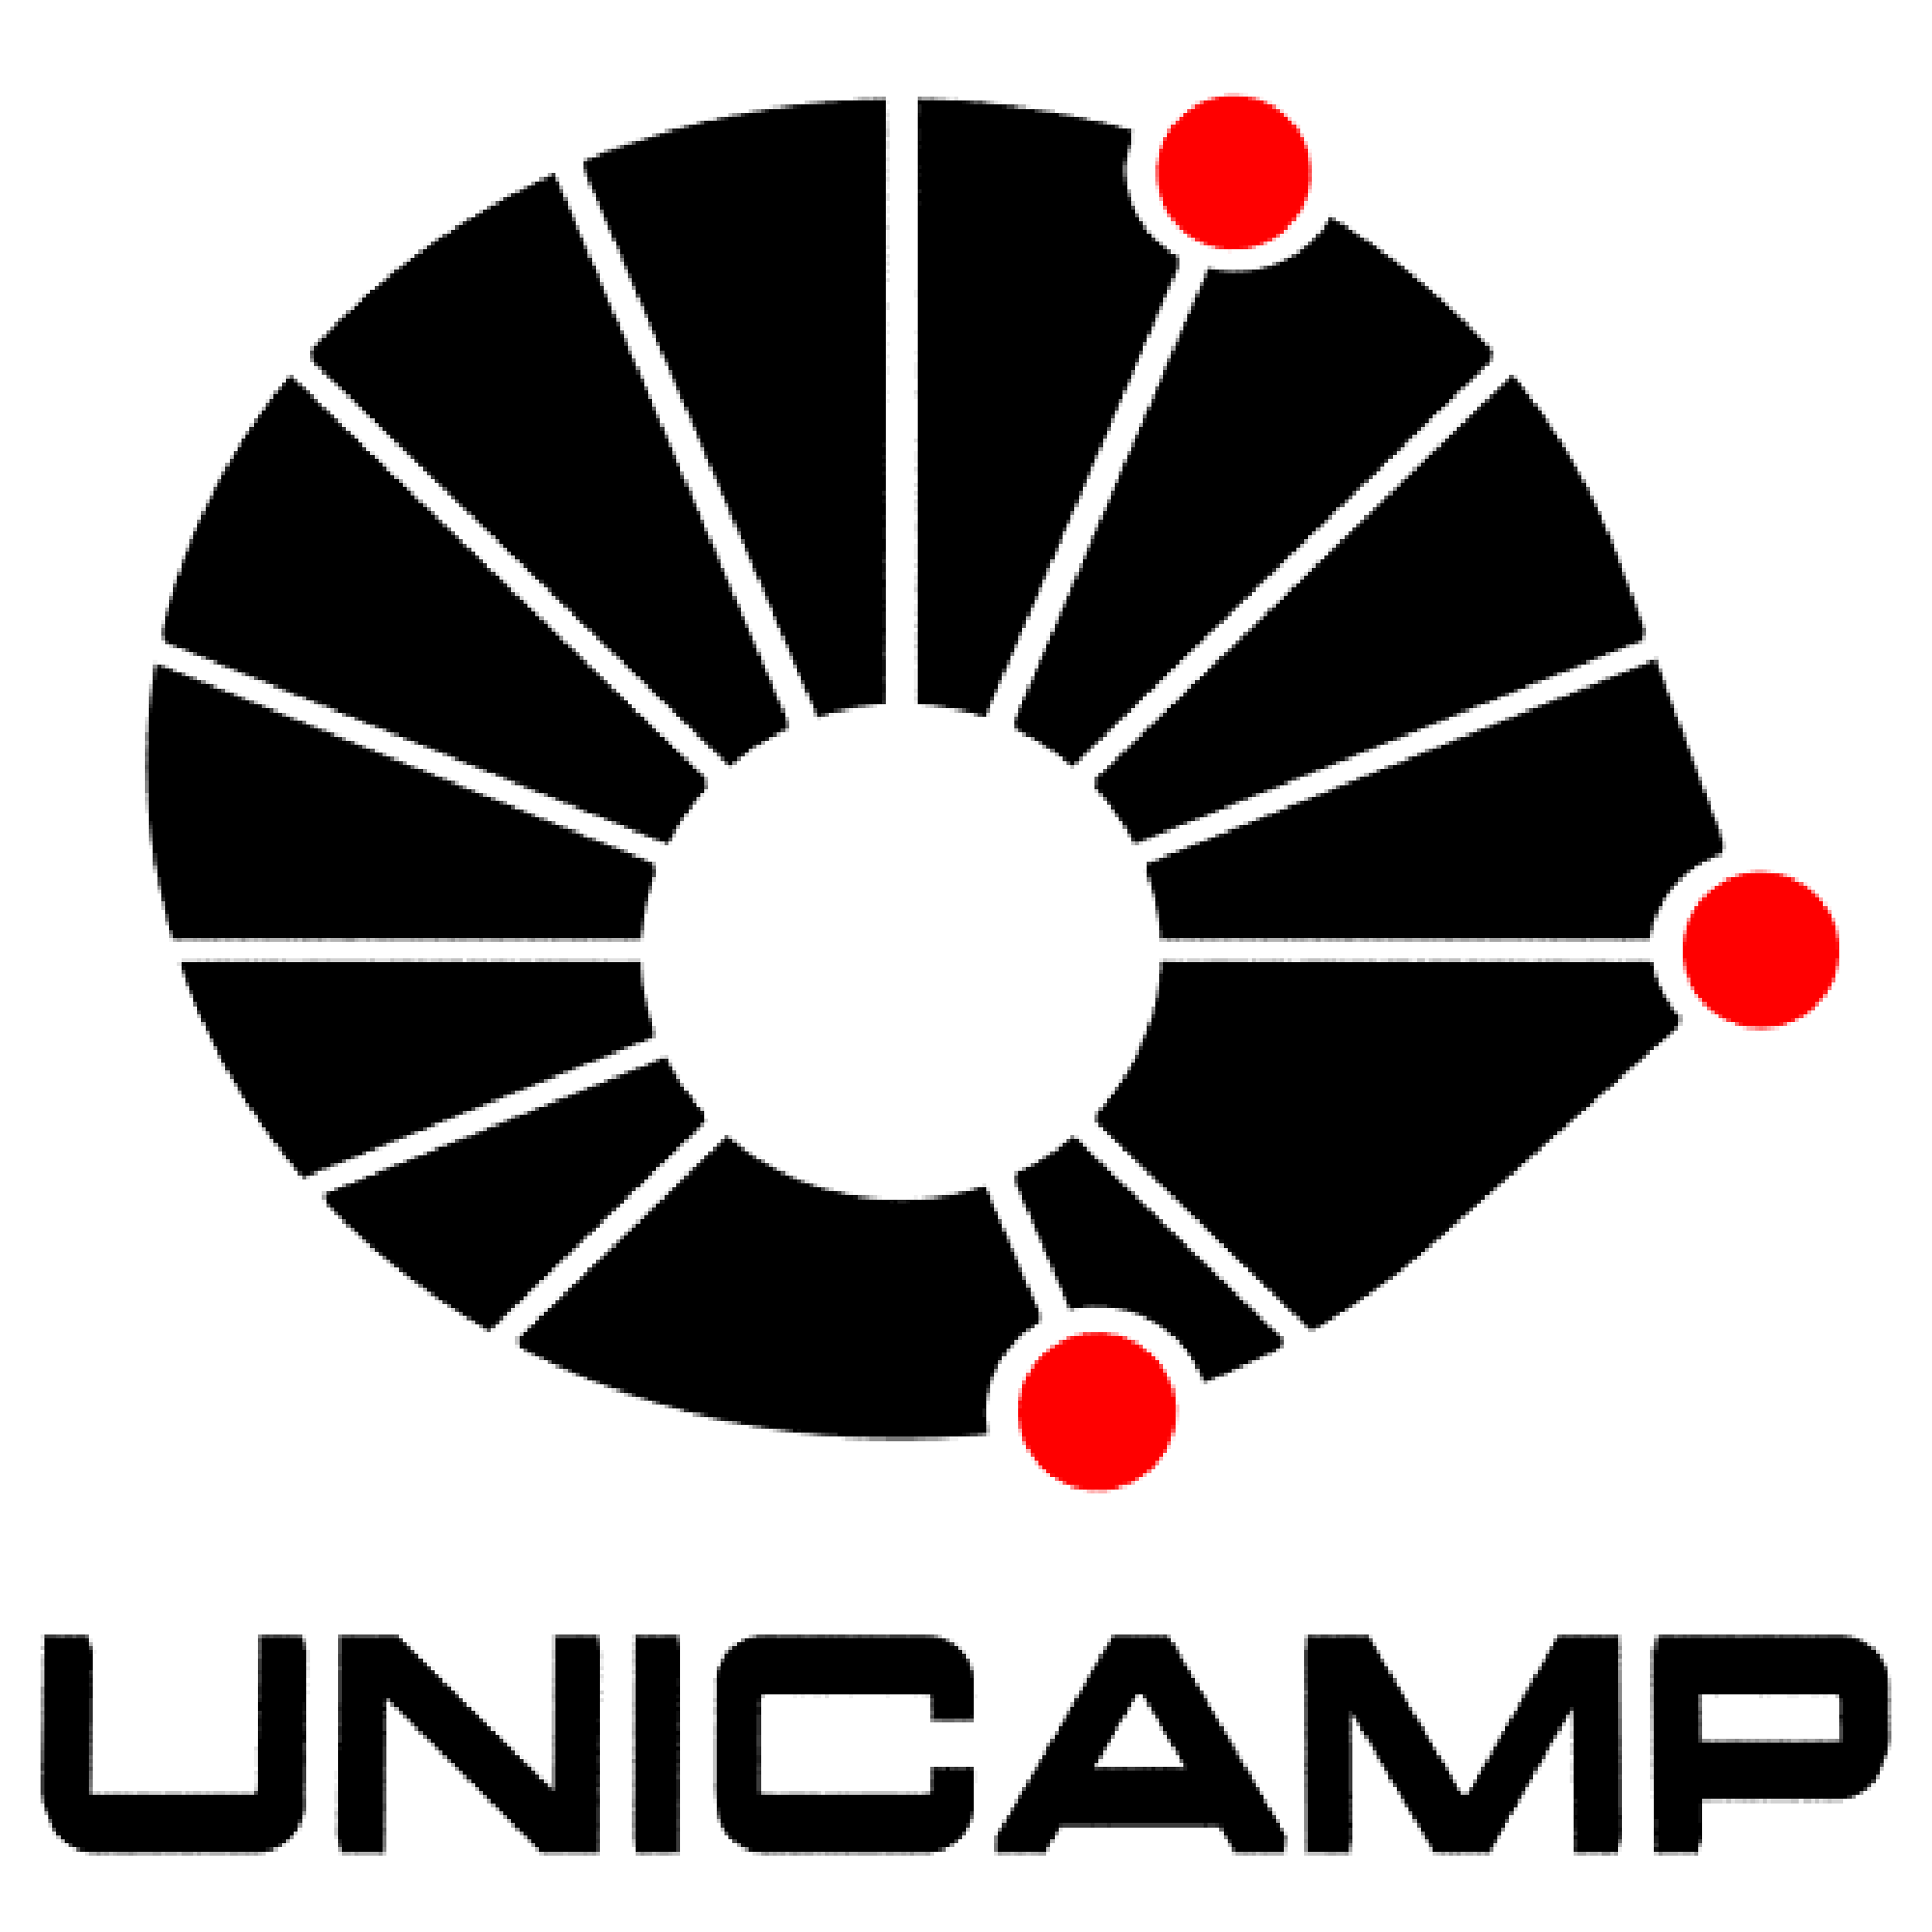
\includegraphics[scale=0.2]{images/logo-unicamp.png}}
% \caption[Shorter figure caption]{Figure Caption caption caption caption
%   caption caption caption caption caption caption caption caption caption
%   caption caption caption caption caption caption caption caption caption
%   caption caption.}
% \label{f:label1}
% \end{figure}
